\documentclass[aps,pra,reprint,onecolumn,12pt,notitlepage,superscriptaddress,nofootinbib]{revtex4-2}
\usepackage[T1]{fontenc}
\usepackage{lmodern}
\usepackage{amsmath,amssymb,bm,graphicx,booktabs}
\usepackage[colorlinks=true,linkcolor=blue,citecolor=blue,urlcolor=blue]{hyperref}
\begin{document}
\title{Production Closure of Derivative-Free Causal Integration in VigilODE:
Exact Constants, Full-Space Certificates, Adversarial Profiles, and Local Qualification}
\author{VigilODE research and implementation audit}
\noaffiliation
\date{27 October 2026 (UTC)}
\begin{abstract}
Starting from PR91, we independently pursue structural stage verification,
scalar homotopy implementation, and selective adapter decisions. No newer PR
was found in the initial remote survey. An exact represented-stage identity
replaces repeated mean-field full-space verification by an outward enclosure
of cost $O(sn+s^2)$, while retaining every state component and charging failed
parallel work. A 2,048-variable, one-worker trajectory has a paired median
speedup of 2.063 and 62.52\% fewer guest instructions than PR91. Scalar
homotopy removes allocation overhead without changing numerical bits; a
proved rational inverse predictor reduces cubic polynomial evaluations from
1,659 to 1,024 under the same physical certificate. The two routes reduce
guest instructions by 36.26\% and 39.01\%, respectively. The adapter's
10.95\% work reduction on one stiff case does not establish a wall-time win;
its reentrant nonlinear alternative remains slower than RHS-only in every
paired block. Exact integer comparison and failure accounting are therefore
kept separate from future-regime optimality. Three, one, and three correction
passes were used for the respective research tasks. A strict serialized
production facade, independent error oracles, native regression checks,
source-bound execution receipts, and a 16-node local development DAG provide
a reviewable deployment setup. General nonlinear closure/order, temporal
residence guarantees, and actual deployment-host release qualification
remain explicit obligations.
\end{abstract}
\maketitle

\section{Scope, prior PRs, and research discipline}
The implementation baseline is commit
\texttt{206298b4068d923bb47c7160b111b7439098660c}, the head of draft PR91
when the work began. The initial GitHub survey inspected the recent 30 PRs
and found no PR newer than 91. PR90 and PR91 remained open drafts, so this
change is prepared on a separate branch stacked above PR91; it does not
merge either predecessor or alter the default branch. The exact survey
receipt and source identities accompany the repository.

The predecessor research is actively reused. PR65's counted common-$W$
corrections warn that sequential forward solves can double work without
shortening the critical path. PR74 and PR75 supply the coupled raw-$U$
target, ordered parallel dispatch, original-residual screening, and charged
speculation. PR77 and the derivative-free originals supply physical
collective/transverse closures. PR90 provides careful prefix-work evidence
and the distinction between residual and physical error. PR91 provides the
exact two-channel mean-field reduction, the dyadic cubic physical-error
plan, exact-input causal reuse, and strict entry selection. Existing SPD04
least-squares workspace reuse is already enabled in the facade; a known
nonnormal Givens differential failure remains an explicit constraint on any
replacement. These contributions are controls and premises, not new claims
of the present report.

Three parallel agents completed separate theory and implementation tracks,
with parent integration and complementary independent native-agent reviews.
The PhysMath Research Loop version 1.0.0 organizes R1--R10 and C1--C10.
Every task records its original target, assumptions, alternatives, exact
derivation, numerical counterprobes, source-bound implementation, actual
tests, and bounded corrections. Shared native builds, timings, and profiles
are serialized by a single lock. Reviewers share project context; their
reviews are not blinded or heterogeneous-model replications.

\begin{table}[tb]
\caption{Separate research tasks and correction budgets. The initial attempt
is recorded separately from a corrective pass. Packaging and environment
repairs are labeled, rather than silently counted as numerical tuning.}
\begin{ruledtabular}
\begin{tabular}{p{.19\textwidth}p{.59\textwidth}r}
Task & Diagnosed target and implemented response & Corrections\\
\hline
Structural & Failed-work loss; repeated full-space residual arithmetic;
adverse scalar cost. Charged API, proved enclosure, exact $n=1$ degeneration. & 3/3\\
Homotopy & Vec/station overhead; costly cubic radicals. Scalar representation
and algebraically derived rational predictor with original certification. & 1/3\\
Adapter & Discarded useful pilot proposals; empirical return margin;
expensive residence in nonlinear regimes. Exact comparisons and causal
proposal reuse, with negative outcomes retained. & 3/3
\end{tabular}
\end{ruledtabular}
\end{table}

The research search used SciSpace for discovery, Exa and primary papers for
source checking, and Wolfram for symbolic identities and independent
inequality checks. No retrieved theorem was treated as a blanket convergence
guarantee for this solver. In particular, modern derivative-free Anderson
acceleration for monotone nonlinear equations has its own projection and
monotonicity assumptions~\cite{JinWangDeng2025}. Historical parallel iterated
RK work separates nonstiff fixed-point iteration from stiff parallel
constructions~\cite{HouwenSommeijer1990,Sommeijer1993}. Neither an implicit
corrector's stability nor a paper's favorable timings transfer automatically
to an arbitrarily truncated causal or homotopy loop.

\section{Evidence hierarchy and main measured outcomes}
The report distinguishes four different objects: a real-arithmetic identity;
a floating-point outward enclosure under declared arithmetic assumptions;
an independent experiment against an original physical target; and a timing
measurement on one host. A smaller projected residual is insufficient for
a full-state conclusion. Fewer callback units need not imply fewer machine
instructions or lower elapsed time. A stage residual bound alone is not a
trajectory accuracy certificate.

\begin{figure}[tb]
\centering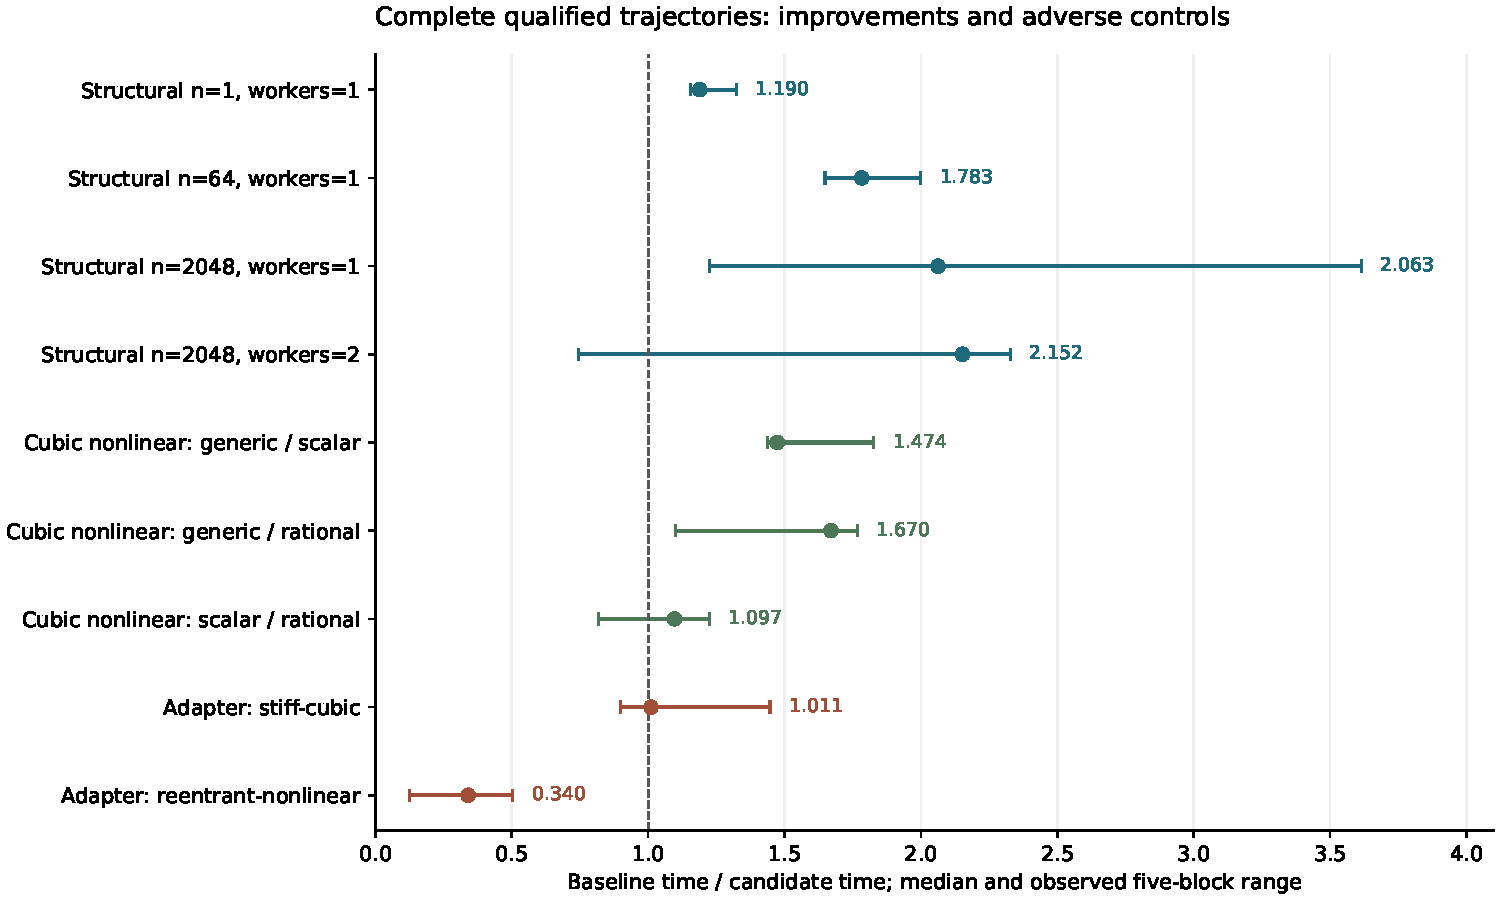
\includegraphics[width=\textwidth]{performance.pdf}
\caption{Measured complete-trajectory speed ratios. Dots are medians of five
ABBA/BAAB blocks; bars are the observed minimum and maximum, not confidence
intervals. Different rows have their explicitly named baselines. The adapter
stiff row compares PR91 with observed proposal reuse; its reentrant row
compares RHS-only with observed proposal reuse and sentinel.}
\label{fig:performance}
\end{figure}

The strongest structural timing observation is the one-worker $n=2048$
enclosure: $2.063\times$, range $[1.226,3.614]$, under the same 64-step
trajectory and physical cap $10^{-6}$. The all-grid states match PR91 bit for
bit. The two-worker range crosses one, so it supplies no general parallel
speed guarantee. A direct fused implementation reduces instructions but
has a negative final one-worker timing median; it remains a measured
alternative rather than the recommended universal choice.

For the nonlinear cubic cohort, generic/scalar and generic/rational medians
are $1.474$ and $1.670$, with all five observed ratios above one. The
scalar/rational ranges cross one in both cubic cohorts. We therefore expose
both strong candidates without installing a fitted runtime threshold.
The recommended scalar Picard representation is a conservative opt-in
implementation choice; the legacy public entry still selects the generic
homotopy. Rational prediction is a separately selectable model-specific
alternative. The original outward physical certificate is retained.

\begin{figure}[tb]
\centering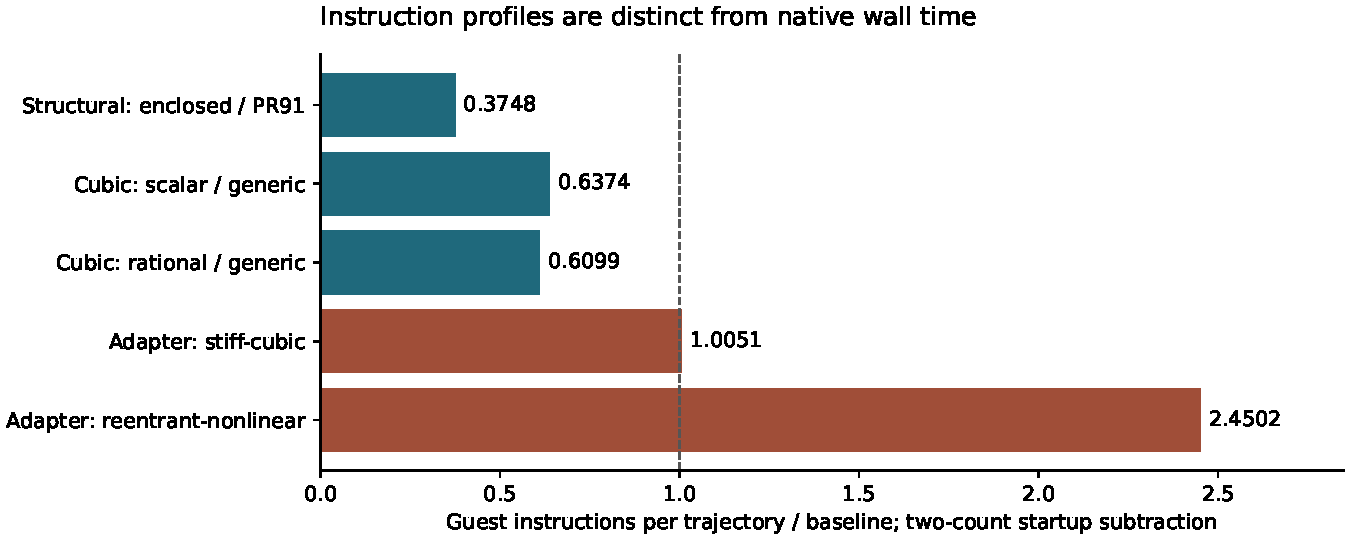
\includegraphics[width=.98\textwidth]{instructions.pdf}
\caption{Startup-subtracted Callgrind instruction ratios from the same
executable within each comparison. These guest instruction counts are
neither hardware cycles nor estimates of end-to-end native wall time.}
\label{fig:instructions}
\end{figure}

The adverse adapter profile is actionable: the adapter dispatcher itself
has negligible self instruction cost, but its decision to remain implicit
incurs norm, QR, orthogonalization and GMRES costs. Optimizing a few
dispatcher branches cannot remove this residence loss. Future work must
separately improve the mode arithmetic and derive when historical evidence
is admissible for later regimes. The current public deployment default is
therefore persistent RHS-only; selective supplied JVP is opt-in.

\section{Structural mean-field closure: charged failures and full-space residual enclosures}
\label{sec:structural-production}

For the immutable affine model
\begin{equation}
 f(y)=b-dy+\kappa\operatorname{mean}(y)\mathbf1,
 \qquad d\ge\kappa\ge0,
\end{equation}
PR91 reduced the original eight-stage raw-$U$ target to two scalar transfer recurrences. The present change preserves every represented stage and endpoint in the successful comparison fixtures. It closes the failed-attempt work contract and replaces repeated full-state verification with a rounding-aware factorization. The model remains derivative-free: no state Jacobian, JVP, state matrix factorization, or Newton update is requested. The shared tableau loader retains its process-lifetime fixed $8\times8$ coefficient inversion; this metadata setup is outside step counters and warmed before paired timing.

\subsection{Original target and exact residual decomposition}
Let $P=\mathbf1\mathbf1^T/n$, $Q=I-P$, $J=-dQ-(d-\kappa)P$, and $a=h\gamma$, with $h>0$ and the fixed tableau's $\gamma>0$. The full original residual is
\begin{equation}
 \mathcal R_i(U)=(I-aJ)U_i-af(y)
 -\sum_{j<i}(\gamma c_{ij}I+a a_{ij}J)U_j.
\end{equation}
All represented input and tableau coefficients are interpreted as exact reals; the enclosure includes the real product $h\gamma$ and real difference $d-\kappa$.

\paragraph{Theorem S1 (represented-stage decomposition).}
For arbitrary $x,\mu$ and transfers $t_i,v_i$, write
\begin{equation}
 U_i=t_i(x-\mu\mathbf1)+v_i\mu\mathbf1+\Delta_i,
 \quad \varepsilon_f=x-f(y),\quad m=\operatorname{mean}(x).
\end{equation}
Define
\begin{align}
 \rho_i(r;z)&=(1+ar)z_i
 -\sum_{j<i}(\gamma c_{ij}-ar a_{ij})z_j-a,\\
 \rho_{ti}&=\rho_i(d;t),\quad
 \rho_{ci}=\rho_i(d-\kappa;v),\quad
 \ell_i=t_i+\sum_{j<i}a_{ij}t_j.
\end{align}
Then
\begin{align}
 \mathcal R_i(U)={}&\rho_{ti}(x-\mu\mathbf1)
 +\rho_{ci}\mu\mathbf1
 +a\kappa\ell_i(\mu-m)\mathbf1+a\varepsilon_f \nonumber\\
 &+(I-aJ)\Delta_i
 -\sum_{j<i}(\gamma c_{ij}I+a a_{ij}J)\Delta_j.
\end{align}
Substitution and $Jx=-dx+\kappa m\mathbf1$ prove the identity. In particular, the transverse factor is $x-\mu\mathbf1$ with the actually computed $\mu$; its discrepancy from the exact projector is explicitly retained. A Wolfram symbolic substitution independently returned a zero vector. The proof applies for arbitrary dimension and arbitrary full-dimensional $\Delta_i$.

\paragraph{Theorem S2 (full original-space bound).}
The exact induced infinity norm of $tQ+cP$ is
\begin{equation}
 \nu_n(t,c)=\left|t+\frac{c-t}{n}\right|
 +(n-1)\left|\frac{c-t}{n}\right|.
\end{equation}
Set
\begin{align}
 w_{ii}&=\nu_n(1+ad,1+a(d-\kappa)),\\
 w_{ij}&=\nu_n(ad a_{ij}-\gamma c_{ij},
 a(d-\kappa)a_{ij}-\gamma c_{ij}),\quad j<i.
\end{align}
If $\|\Delta_j\|_\infty\le\delta_j$,
$\|\varepsilon_f\|_\infty\le\epsilon$,
$|\mu-m|\le\zeta$, and $\|x-\mu\mathbf1\|_\infty\le X$, then
\begin{equation}
 \|\mathcal R_i(U)\|_\infty\le
 |\rho_{ti}|X+|\rho_{ci}|\,|\mu|
 +|a\kappa\ell_i|\zeta+a\epsilon
 +\sum_{j\le i}w_{ij}\delta_j.
\end{equation}
This follows directly from S1 and the induced norm inequality. Every scalar coefficient, block norm and nonnegative final accumulation is enclosed outward. The bound covers all $8n$ original residual components at cost $O(sn+s^2)$ instead of $O(s^2n)$. Only the individual block norm is asserted sharp; the combined rounding envelope is generally conservative.

\subsection{Rounding constants and scalar specialization}
\paragraph{Theorem S3 (operation-wise rounding enclosure).}
The arithmetic assumptions are binary64 round-to-nearest, gradual underflow, finite intermediates, and no unsafe reassociation. Let $r(z)$ be half the binade spacing at a finite rounded result, rounded upward to the least positive subnormal when necessary. This is the round-to-nearest error radius; it is derived from the exponent, with no fitted factor.

For the existing scaled Neumaier mean, put $s=\operatorname{fl}(1/n)$, $v_i=\operatorname{fl}(s x_i)$ and let $C_i$ be the accumulated compensation. FastTwoSum supplies exact local addition residuals~\cite{OgitaRumpOishi2005}. Upward sums
\begin{equation}
 A\ge\sum_i|v_i|,\quad E_p\ge\sum_i r(v_i),\quad
 E_c\ge\sum_i r(C_i),\quad \theta\ge r(s)/s
\end{equation}
yield
\begin{equation}
 |\widehat m-\operatorname{mean}(x)|
 \le E_p+\theta(A+E_p)+E_c+r(\widehat m).
\end{equation}
Telescoping the exact local corrections proves the accumulation part; the remaining two terms bound scaled-product and reciprocal error. The enclosure plan requires an exactly represented positive integer dimension at most $2^{53}$.

For an actual stage lift
$p=\operatorname{fl}(t_i\operatorname{fl}(x_k-\mu))$,
$q=\operatorname{fl}(v_i\mu)$ and
$U_{ik}=\operatorname{fl}(p+q)$, the sum of the four local error bounds gives
\begin{equation}
 \|\Delta_i\|_\infty\le\delta_i:=r(\max_k|U_{ik}|)+r(\max_k|p_k|)+r(q)
 +|t_i|r(\max_k|\operatorname{fl}(x_k-\mu)|).
\end{equation}
The affine RHS is enclosed from its represented product, subtraction, shared mean term and final addition in the same way.

\paragraph{Theorem S4 (exact scalar degeneration).}
For $n=1$, $P=I$ and $\mu=x$ exactly. Consequently the real represented stage is one rounded product $U_i=\operatorname{fl}(v_i x)$, together with exact signed-zero operations retained for bit compatibility. With $u=2^{-53}$ and $\eta=2^{-1074}$,
\begin{equation}
 |\operatorname{fl}(z)-z|\le u|z|+\eta/2.
\end{equation}
The unrepresentable positive $\eta/2$ is enclosed upward by $\eta$. Therefore
\begin{equation}
 |\mathcal R_i(U)|\le
 \left(|\rho_{ci}|+u\sum_{j\le i}w_{ij}|v_j|\right)|x|
 +\eta\sum_{j\le i}w_{ij}+a\epsilon.
\end{equation}
The two sums are plan-only quantities and are precomputed outward, reducing per-step scalar verification to $O(s)$. The special case is the exact projector degeneration, not a measured dimension cutoff.

\subsection{Failure accounting and comparison design}
The new charged methods return \texttt{StructuralFailure\{error,work\}}. Scheduler closures return each stage result as data, all jobs are joined, their actual work is accumulated, and the first failure in stage order is returned. A failed job cannot cancel another scheduled job's accounting. Pre-attempt refusals retain zero work. Legacy method signatures remain available; adaptive clients use the charged variants.

Two implementations were compared against the byte-identical PR91 source in the same executable. The fused direct screen removes two full-state temporary vectors while preserving the original arithmetic order. The factorized screen supplies an outward bound and refuses when that bound exceeds the original requested limit. Full 64-step trajectories retain the original physical cap $10^{-6}$, same-target cap $10^{-11}$ and residual cap $10^{-9}$. Every observed state was bit-identical to PR91.

\begin{table}[tb]
\caption{Final paired full-trajectory timings versus PR91. Values are medians of five ABBA/BAAB blocks with their observed ranges, not confidence intervals. Model allocation, plan construction, stages, screening, endpoint and return allocations are timed.}
\begin{ruledtabular}
\begin{tabular}{rrll}
$n$ & workers & fused direct & factorized enclosure\\
\hline
1 & 1 & $1.011\ [0.737,1.231]$ & $1.190\ [1.154,1.323]$\\
64 & 1 & $1.168\ [0.915,1.266]$ & $1.783\ [1.649,1.998]$\\
2048 & 1 & $0.840\ [0.619,1.220]$ & $2.063\ [1.226,3.614]$\\
2048 & 2 & $1.213\ [1.032,1.276]$ & $2.152\ [0.745,2.328]$\\
\end{tabular}
\end{ruledtabular}
\label{tab:structural-closure}
\end{table}

At $n=2048$, complete-trajectory RHS evaluations fell from 576 to 64, physical linear actions from 512 to zero, and causal full-state accumulations from 7,340,032 to zero. All 1,048,576 stage residual components remain covered; 262,144 mean components and 1,048,576 lift components receive explicit rounding enclosures. The maximum grid error is unchanged at $2.398\times10^{-10}$.

The initially unfavorable scalar result was retained: before the last correction, the enclosure gave $0.392\times$ and the charged fused implementation $0.694\times$ in five paired blocks. The exact $P=I$ specialization and algebraic aggregation of batch work address that diagnosed cost. The final scalar enclosure gives $1.190\times$. This is a post-diagnostic improvement; final large-case fused timing remains uncertain and its negative median is reported.

Eleven distinct native contracts pass (five reused structural contracts and six new production contracts). Independent exact-rational evaluation of the full original equations confirms 168 stage bounds across 21 fixtures and 728 residual components, including large cancellation, nonrepresentable rate differences and subnormals. The 8,184 exponent-wide checks of round-to-nearest radii are reused after the scalar update. Three correction passes were used: crate-local control packaging, a portable integer dimension guard, and the diagnosed scalar/accounting optimization. No further solver tuning was performed.

A final Callgrind 3.22.0 profile used two and six complete trajectories per arm at $n=2048$, one worker, and subtracted startup via $(I_r(6)-I_r(2))/4$. All six runs exited zero with unchanged source and binary. Instructions per trajectory were $347{,}516{,}244.75$ for PR91, $309{,}511{,}284.25$ for fused direct, and $130{,}256{,}982$ for the enclosure: reductions of $10.94\%$ and $62.52\%$, respectively. These guest instruction counts are reported separately from native wall time; the fused timing median remains negative in the final large single-worker sample. Protocol, commands, raw profiles and hashes are retained in \texttt{instruction\_profile/}.

The certificate concerns original stage residuals. A complete outward physical trajectory certificate still requires outward propagation constants, temporal truncation and endpoint-rounding contributions. These are explicit local follow-up obligations; the current measured trajectory accuracy and stage certificate are separate evidence.

\section{RHS-only scalar closure and certified inverse candidates}
The sealed consumer solves $y'=-ky-gy^3$, with $k>0$, $g\geq0$ and
$y(0)=Y\geq0$.  Its PR91 dyadic plan, finite-step truncation coefficient
$C=(k+3gY^2)^2(kY+gY^3)/8$, and outward physical certificate are unchanged.
Candidate generation is now selectable: the original generic homotopy,
a stack-valued scalar specialization, a positive-sum cubic inverse, and a
rational inverse predictor.  The generic public entry point is retained.

\paragraph{Exact inverse representation.}
For the midpoint equation $am+bm^3=y$, put
\begin{align}
 a&=1+hk/2,& b&=hg/2,& \beta&=by^2/a^3,\\
 z&=\tfrac32\sqrt{3\beta},&
 u&=(z+\sqrt{1+z^2})^{1/3},&
 s&=\frac{3}{u^2+1+u^{-2}}.
\end{align}
Then $m=(y/a)s$ is the unique real solution.  Indeed, the polynomial is
strictly increasing.  For $\beta>0$, $u^3-u^{-3}=2z$ and
\begin{equation}
 (u-u^{-1})(u^2+1+u^{-2})=2z
\end{equation}
give $s=(u-u^{-1})/\sqrt{3\beta}$.  The identity
$(u-u^{-1})^3+3(u-u^{-1})=u^3-u^{-3}$ proves $s+\beta s^3=1$.
At $\beta=0$, the positive-sum formula directly gives $s=1$.
The existing contraction domain gives $0\leq\beta<1/3$ and $0\leq z<3/2$.
No subtraction of nearly equal cube roots is required.

\paragraph{Rational alternative and its defect.}
The inverse series starts $1-\beta+3\beta^2$.  Matching a $[1/1]$
rational expression uniquely determines
\begin{equation}
 r(\beta)=\frac{1+2\beta}{1+3\beta},\qquad
 r+\beta r^3-1=\frac{\beta^3(3+8\beta)}{(1+3\beta)^3}.
\end{equation}
The right-hand side is nonnegative for every $\beta\geq0$.  Since the
residual derivative is $1+3\beta s^2\geq1$, its unique positive root $s_*$
satisfies
\begin{equation}
 0\leq r-s_*\leq\frac{\beta^3(3+8\beta)}{(1+3\beta)^3}.
\end{equation}
These coefficients follow from algebra; none was fitted to timing data.
Wolfram symbolic evaluation and 151 exact rational cells for each identity
provide independent checks of the displayed formulas.

\paragraph{Original-target certificate.}
Both inverse candidates form the increment as $\widehat K=-h\phi(\widehat m)$,
avoiding the subtraction $2(\widehat m-y)$.  Their floating-point accuracy is
not assumed.  Acceptance evaluates the original
$F(K)=K+h\phi(y+K/2)$ in outward intervals.  For every real $K$,
$F'(K)\geq D=1+hk/2$, hence
\begin{equation}
 |\widehat K-K_*|\leq |F(\widehat K)|/D.
\end{equation}
Adding the enclosed represented-update displacement preserves the previous
nonexpansive physical-error induction.  A missed budget invokes charged scalar
Picard and, if needed, the existing monotone bisection.  A rounding-floor
refusal preserves the accepted prefix.  Predictor counts are reported
separately from ordinary and interval polynomial evaluations.

\paragraph{Representation and measured costs.}
The scalar specialization preserves operation order, seed, actual residual
screen, and all charged callback evaluations.  Forty combinations of model,
mode and seed policy preserve every returned state and error-bound bit.
Twenty-three distinct native contracts pass.  The final 24 accuracy arms,
containing 5,404 returned observations, satisfy the unchanged native outward
bound under an independent Decimal80 exact-ODE oracle.

For $k=1$, $g=1/2$, $Y=T=1$, Table~\ref{tab:production-cubic-work} compares
warm Picard against the rational predictor.  Scalar Picard has the same
work and output bits as generic Picard. The final outward bound in the
tight rational case is $4.46606\,10^{-6}$.
\begin{table}[ht]
\caption{Identical physical accuracy plans.  Each rational step also performs
one separately counted rational inverse calculation.}
\label{tab:production-cubic-work}
\begin{ruledtabular}
\begin{tabular}{rrrrr}
$\epsilon$ & $N$ & Picard RHS+interval & Rational RHS+interval & \shortstack{Rational\\max. error}\\
\hline
$10^{-3}$&64&198&128&$1.43850\,10^{-5}$\\
$10^{-4}$&128&462&256&$3.59356\,10^{-6}$\\
$10^{-5}$&512&1659&1024&$2.24475\,10^{-7}$
\end{tabular}
\end{ruledtabular}
\end{table}
Same-binary Callgrind differences between 20 and 40 complete trajectories
give instruction slopes 3,182,149.3 (generic), 2,028,310 (scalar),
2,061,615 (algebraic), and 1,940,807 (rational).  Scalar and rational reduce
this measure by 36.26\% and 39.01\%, respectively.  Rational is 4.31\% below
the strong scalar implementation.  These are guest instructions with process
startup subtracted, not hardware cycles.

Five paired ABBA/BAAB wall-time blocks include full output allocation and
all interval verification.  Generic/scalar median ratios are 1.728 for the
baseline cubic and 1.474 for the nonlinear-dominated fixture.  Corresponding
generic/rational medians are 1.514 and 1.670.  Scalar/rational medians are
0.970 and 1.097, with observed ranges crossing unity; local hardware selection
between these strong alternatives remains warranted.  The expensive cubic
inverse was the diagnosed adverse alternative.  Exactly one corrective loop
introduced the rational predictor, and all initial negative measurements remain.

The original physical certificate is retained in every comparison.  Its
\texttt{Interval::mul} instruction count is unchanged and accounts for 55.06\%
of the rational profile.  Improving the finite-step truncation estimate and
vector-valued homotopy workspace are separate subsequent research tasks.

\section{Adapter selection and mode arithmetic are separate costs}
\label{sec:production-adapter}

The adapter now offers exact integer return selection and causal transport
of an observed entry-step proposal. Both new flags default to false.
The general production configuration retains persistent RHS-only execution;
supplied-JVP fallback is an explicitly qualified option. The measured adverse
cases below are retained in the release evidence.

Let
\begin{equation}
 W=N_f+N_{Jv}+N_{f_t}+nN_J+N_{\mathrm{solve}}.
\end{equation}
This is the existing accounting objective. For a completed explicit
candidate of work $E$ and a same-window implicit incumbent of work $I$,
strict improvement is exactly $E<I$. If the implicit replay is incomplete,
its charged nonfatal prefix $L$ proves the same preference when $E<L\le I$.
The implementation checks the complete candidate and finite window identity,
then compares checked \texttt{u128} sums; ties retain the incumbent.

\paragraph{Exact stopping constants.}
The native callback guard charges the crossing callback before stopping at
$L_{\rm cb}>\mathrm{cap}$. Consequently, a completed explicit candidate
requires an implicit-comparator cap $E$: crossing proves $E<L_{\rm cb}\le I$.
A productive implicit sentinel of cost $I$ instead bounds its explicit
challenger by $I-1$. Crossing then makes a strict explicit win impossible.
These integer boundaries follow from the comparison objective rather than
an empirical gain margin. Since a native DOPRI attempt performs at most seven
RHS calls, the sentinel has
\begin{equation}
 W_{\rm sentinel}\le 2I+6,\qquad I\ge1.
\end{equation}
This is an overhead bound relative to the current implicit window, whose
cost can itself be unfavorable.

\paragraph{Causal proposal transport.}
An earlier nonfatal pilot with $m>0$ accepted steps from $a$ to $c>a$
provides $\bar h=(c-a)/m$. A later pilot may use
$\max(h_0,h_{\rm checkpoint},\bar h)$, clipped to its native replay interval,
while retaining the later accepted physical state and every native error
and work test. This transports a past scalar proposal; route selection still
requires a fresh successful cost comparison. Zero-accepted and fatal pilots
provide no proposal. Forty-four actual pilot initializations satisfy this
causal formula in the recorded trajectories.

\paragraph{Nonlinear exact-state tests.}
For the autonomous augmentation $c'=1$ and
\begin{equation}
 y_j'=-\lambda(c)(e_j+e_j^3/2)+g'(c),\qquad e_j=y_j-g(c),
\end{equation}
separation with $z=e_j^{-2}$ gives $z'=2\lambda z+\lambda$ and hence
\begin{equation}
 e_j(t)=\frac{e_j(0)e^{-\Lambda(t)}}{
 \sqrt{1+e_j(0)^2[1-e^{-2\Lambda(t)}]/2}},\qquad
 \Lambda(t)=\int_0^t\lambda(s)\,ds.
\end{equation}
The constant, relaxing and reentrant rates have explicit $\Lambda$ through
$\log\cosh$. Independent Decimal90 evaluation checks all 17,440 returned
state components. Exact rational Laurent-polynomial arithmetic verifies the
inverse-square transformation and the supplied directional Jacobian action.
All 36 arms pass their original accuracy and callback-accounting contracts.

\begin{table}[tb]
\caption{Whole-trajectory charged work. All discarded pilots and return
probes are included. ``Observed'' transports the accepted pilot-step mean.}
\label{tab:production-adapter-work}
\begin{ruledtabular}
\begin{tabular}{lrrrr}
Case & RHS-only & PR91 & Observed & Observed+sentinel\\
Easy cubic &79&79&79&79\\
Stiff cubic &2347&2958&2634&2634\\
Relaxing nonlinear &10375&11407&16331&12195\\
Reentrant nonlinear &17113&18600&27546&24440
\end{tabular}
\end{ruledtabular}
\end{table}

The original 20-arm test produced no selective switches: a completed pilot
could cost 204 against 192 explicit units, and its useful accepted step was
discarded. The observed-step correction enables entry, but Table~\ref{tab:production-adapter-work}
shows that this can increase total work after a regime change. Sentinel
returns recover part of that loss. Exact and ratio-based return decisions
coincide on this physical cohort; integer near-tie tests distinguish their
decision boundaries separately.

\begin{table}[tb]
\caption{Paired timing and instruction slopes for complete qualified
trajectories. Ranges are five observed block ranges, not confidence intervals.}
\label{tab:production-adapter-profile}
\begin{ruledtabular}
\begin{tabular}{lrr}
Comparison &Instruction change&Median speedup [range]\\
Stiff: PR91 to observed & $+0.505\%$ &1.0106 [0.8981,1.4469]\\
Reentrant: RHS-only to sentinel &$+145.02\%$&0.3404 [0.1265,0.5046]
\end{tabular}
\end{ruledtabular}
\end{table}

Five ABBA/BAAB blocks, recorded before the final branch-style cleanup, use
one fixed measured executable and 64 full solves per process for stiff cubic and 16
for reentrant relaxation. Model and result allocation are timed; exact-state
analysis and JSON serialization follow the timer. Callgrind differences
between four and twelve repeated solves remove fixed startup/output cost.
The stiff-cubic work decrease of $10.95\%$ does not produce a stable measured
time improvement. The reentrant selective route is slower in every paired
block. In its twelve-solve profile, dispatch function
\texttt{drive\_windows} has only $0.0225\%$ self instructions, whereas
\texttt{safe\_l2}, pivoted QR, two-pass MGS and GMRES account for
$9.77\%$, $3.72\%$, $3.53\%$ and $2.63\%$, respectively. These self costs
identify mode arithmetic separately from the adapter's choice of which
mode to execute.

Thirty-five distinct native contracts pass. Three correction passes were used:
observed-step transport after the negative initial cohort, then initialization
of its new field in an existing private test fixture, and finally two equivalent
let-chain rewrites required by production CI. The final rewrite preserves
left-to-right short-circuit evaluation and changes no policy, numerical
constant or fixture. Historical timing and profiling retain their original
source and executable identities. Fatal-callback priority,
accepted-prefix preservation, strict integer boundaries, forbidden derivative
work, configuration serialization and all prior relevant return contracts
remain tested. The final 36-arm correctness audit exactly reproduces all
17,440 state components, counters and segment decisions in the earlier
records; only elapsed time is excluded from the comparison and the original
missing default-false option is normalized. Existing high-precision oracle
evidence is reused on these identical inputs. No final-source paired timing
or instruction measurement is inferred from that equality. Further
development must address cost intervals for small
Krylov arithmetic, quantified residence loss under changing regimes, and
complete native-session transfer after winning explicit probes.


\section{What is a mathematical gap, and what is code optimization?}
The following division is based on the claims required by each route.
It does not infer a strong impossibility theorem from a finite failed
experiment. A restricted construction can remain useful while a broader
claim is unsupported.

\subsection{Structural closure and a physical trajectory theorem}
The affine mean-field quotient is exact because the declared operator
preserves the span of the collective and transverse projectors. Its
arbitrary full-state forcing is retained. Repeated full-state verification
was consequently an implementation bottleneck with a constructive exact
factorization. Rounding, however, means that a computed mean is not the
exact projector and a lifted stage is not the exact two-channel state.
Theorem S1 supplies the missing terms, and S2--S4 turn them into an
executable enclosure. Discarding these terms would have been a mathematical
defect in a certificate, not merely an inefficient implementation.

The new stage certificate still does not establish an outward physical
trajectory bound. The old accumulated algebraic budget is evaluated in
ordinary binary64, and time truncation, endpoint addition and observation
time errors have independent contributions. A variable-step extension must
derive the adjoint/product residual transport, bound every rounding term,
and state its operator-commutation conditions. A nonlinear extension must
bound the closure remainder on an explicit invariant domain. PR-N03 carries
these proof obligations before an adaptive consumer can claim a physical
certificate.

\subsection{Causal parallelism and high-order nonlinear carriers}
The finite triangular target admits exact forward substitution and finite
causal propagation. These statements establish neither cheap parallel
execution nor the high-order conditions of a changing nonlinear carrier.
The inherited general causal path still uses a frozen JVP basis and small
projected linear algebra; calling it universally derivative- or matrix-free
would be incorrect. Exact cache identity and buffer reuse are implementation
tasks. Proving original-space residual amplification, closure remainders,
and order under carrier rebuilding is a theory task.

The relevant performance comparison includes total work and critical path.
Independent stage or model jobs can execute concurrently, but communication,
validation, pool startup and the best forward solve are part of the
comparison. PR-N05 keeps that strong serial baseline and an explicit
work/span contract. The existing successful structural special case is
evidence for this restricted algebra, not a general proof that sequential
RK dependencies can always be removed profitably.

\subsection{Root finding, certificates, and remaining accuracy cost}
The scalar representation is a direct code optimization: fixed arithmetic
order and 40 mode/seed/model comparisons establish bit parity. The rational
inverse is a constructive algebraic alternative whose coefficients and
defect are proved. Its acceptance continues to use the original equation,
so no unproved libm cube-root accuracy is trusted. The specific monotone
cubic model supplies existence, uniqueness, a bracket and a residual-to-root
constant. A generic nonlinear homotopy needs its own branch, domain,
monotonicity or inverse-control assumptions. Without them, the finite-budget
failure contract remains explicit.

After root-cost reduction, interval multiplication accounts for 55.06\%
of the rational instruction profile. Removing certificate work without a
replacement proof would relax the scientific target. PR-N02 instead seeks
a tighter finite-step defect along the actual decay envelope, an outward
sum of propagated error, and the smallest admitted grid. This targets
the number of certified steps, while generic vector workspace reuse in
PR-N04 targets allocation. Their savings must be attributed separately.

\subsection{Selection evidence and future regimes}
Exact integer comparison proves a current same-target work preference.
The $2I+6$ sentinel theorem bounds current-window overhead relative to its
implicit incumbent. Neither statement bounds the incumbent's future cost.
The measured reentrant loss demonstrates the gap between the selector's
proxy and actual full-trajectory cost in this cohort. It is not a theorem
that derivative-free or selective methods are universally inferior.

A defensible future-regime claim must assume a quantitative variation,
dwell-time or model-domain condition, define evidence epochs, and charge
exploration and invalidated probes. PR-N06 is distinct from the arithmetic
cost model in PR-N01. It seeks a finite-horizon residence/exploration bound
and budget-derived revalidation rules. An empirical multiplier without
such a theorem would not meet the requested exact-constant standard.

\subsection{Constants and caller choices}
New method constants have an explicit origin: $2$ and $3$ in the rational
inverse arise from series matching; $1+hk/2$ is the exact strong-monotonicity
lower bound; the structural block weight is an induced norm; $2^{-53}$ and
$2^{-1074}$ are binary64 arithmetic constants; the adapter's $I-1$, $E$ and
$2I+6$ follow from integer strictness and native attempt overshoot. None is
a fitted hyperparameter.

This does not erase legitimate user inputs. Physical tolerances, initial
step proposals, thread count, attempt/resource caps and observation windows
belong to the client or execution environment. Existing controller and
pressure/backoff policy constants are preserved operational choices, not
newly proved universal optima. The JSON templates use one declared smoke
fixture and label these inputs accordingly. A claim that every inherited
hyperparameter has been eliminated would exceed the work performed.

\section{Production configuration and failure-preserving execution}
The additive public API exports \texttt{ProductionConfig},
\texttt{ProductionSolver}, and schema version one. The default factory
selects persistent RHS-only execution. The selective factory accepts only
a supplied JVP, requires replay-safe callbacks, preserves the explicit
session, and installs strict entry and return evidence. It does not
automatically enable observed-step reuse or one-window sentinel probing.
Unsupported derivative permissions and incomplete configuration are
rejected before callbacks run.

Strict deserialization covers the top level, switching configuration,
nested options and absolute tolerance. Unknown fields such as a misspelled
step limit are rejected. The legacy general \texttt{Options}
deserialization behavior is unchanged; production uses a strict
intermediate representation. Native feature validation continues to govern
mass matrices, nonautonomous time derivatives, dense output, events and
tolerance combinations. This is an endpoint-oriented smooth forward
identity-mass setup, not a promise that every experimental route supports
every facade feature.

The result retains success, reached time, method segments, actual callback
work, accounting completeness and an accepted prefix on numerical failure.
Callers inspect these fields instead of equating an outer successful return
with a completed integration. Charged structural APIs are required for new
adaptive or retrying consumers; legacy wrappers intentionally discard only
the failure work payload for signature compatibility. A callback panic
under an aborting process profile cannot fulfill a returned partial-result
contract. Expected model failures should use the declared callback error.

The executable \texttt{production\_from\_json} emits complete templates and
reads them back. On $n=16$, $y'=-r y$, $[0,1]$, four combinations of
RHS-only/selective and $r=1,1000$ pass the original $10^{-6}$ all-returned-state
cap and atomic work accounting. The RHS-only cases make zero JVP calls.
The stiff selective case records 1,117 RHS and 426 JVP calls against 2,377
RHS calls in the default case; its observed accuracy is
$1.0654\times10^{-9}$. This controlled smoke result does not override the
adverse nonlinear adapter evidence.

\section{Validation, reproducibility, and interpretation limits}
The full facade and coupled native test sets pass 297 and 127 tests,
respectively, with zero failed or ignored tests in the final invocation
after the integration-accounting repair described below.
The narrower lane counts (11 structural, 23 homotopy, 35 adapter and five
production-setup contracts) overlap those complete package sets and are
not added again. All-target compilation, warning-free rustdoc and two
doctests are checked separately. Final integration gate receipts and any
later format-only qualification are authoritative in
\texttt{evidence/VALIDATION\_SUMMARY.json}; they distinguish tests from
compilation, linting and publishing.

The broader five-package invocation exposed an inherited lagged-GMRES
accounting defect after 1,312 passing tests, one failure and 45 ignored tests.
The solver-level counter already charged attempted operator applications,
whereas the physical work hook charged successful completions. With $A$
entered applications and $P$ charged physical applications, the missing
physical work is exactly $A-P$ for representable counters. Reconciliation
against the attempted-operator count had incorrectly yielded zero for a
failed JVP. The local repair separates these ledgers, leaving callbacks,
numerical arithmetic, tolerances and the original failing assertion unchanged.
The original regression and successful dense/JVP contracts then pass.
The recorded post-repair scope covers eight reachable lagged targets and
the complete facade/coupled sets: 464 distinct tests pass, none fail,
and four measurement tests remain ignored. This is not a fresh successful five-package
sweep. Unrelated exact-oracle evidence is reused through source and route
identity. Full deployment release qualification remains a local gate.

Independent oracles include 728 exact full structural residual components
and 168 stage bounds across 21 fixtures; 5,404 cubic grid observations
against Decimal80; and 17,440 nonlinear adapter state components against
Decimal90. Exact-rational symbolic checks and Wolfram receipts accompany
the proofs. The unchanged structural rounding-radius routine reuses 8,184
exponent/mantissa checks. Finite checks supplement the displayed proofs;
they do not establish unrestricted floating-point correctness by sampling.

The shared host uses an Intel Xeon Platinum 8573C, nine logical CPUs in
the affinity set, an eight-core CPU quota and an 8-GiB memory limit.
Rust 1.94.1 and the locked dependency graph are pinned. Cloud measurements
use opt-level three, no LTO and 16 codegen units. Deployment qualification
uses the existing release profile with fat LTO and one codegen unit.
Those profiles and their binary hashes must not be mixed. Native timings
are descriptive paired observations on a shared host. Oracle evaluation and
JSON serialization are outside the recorded timer; the relevant model,
plan, solve, validation and return allocation costs are included as stated
in each protocol. Thread-pool construction is reported separately.

The new command recorder binds actual argv, environment, source/input hashes,
executable identity, stdout/stderr hashes, timeout and exit status. Source
discovery is repeated after execution, so new files also invalidate a
qualification. A successful command with changed source is recorded as
stale and returns failure. Owned process groups are cleaned on timeout,
cancellation and direct-child completion before the suite lock is released.
Seven actual toy-process contracts exercise success, nonzero exit, missing
executable, modified/new input and resistant-grandchild timeout/cancellation.
Code review covers the spawn and lock races; those tests do not exhaust all
scheduler interleavings.

The initial negative cohorts, compile-time fixture failure, profiler
environment preflight failure, and unfavorable final measurements are
retained. Environment repairs do not become numerical improvement claims.
Raw evidence is stored with a per-member hash manifest and reproducible
archive, alongside the final source manifest. The package verifier checks
identity and DAG consistency; its pass is a packaging result, not a
mathematical proof or a deployment certificate.

\section{Local development DAG and PR contracts}
The machine-readable plan contains 16 nodes and eight executable suites.
The completed remote survey feeds the three research lanes; those feed
production integration, cloud validation, and publication. Local release
verification precedes hardware measurements. Four development branches can
then pursue independent scoped work. Native timing and profiling stay
serialized even when proofs and disjoint edits run concurrently.

\begin{table}[tb]
\caption{Future local PR contracts. Every research PR starts with its own
unchanged target and at most three corrective passes. The JSON plan includes
code targets, expected artifacts, reuse links and explicit acceptance tests.}
\begin{ruledtabular}
\begin{tabular}{p{.18\textwidth}p{.25\textwidth}p{.44\textwidth}}
Node & Prerequisite & Purpose and required evidence\\
\hline
PR-N01 & L-HARDWARE & Small Krylov norm/QR/MGS cost; retain existing LS
workspace; prove true-residual and rank/breakdown conditions.\\
PR-N02 & L-RELEASE & Finite-step cubic bound on the decay envelope;
outward error sum and smallest admitted grid.\\
PR-N03 & L-RELEASE & Variable-step transport, temporal truncation and
endpoint rounding; charged adaptive consumption.\\
PR-N04 & L-RELEASE & Complete session/epoch transfer and generic vector
homotopy workspace with preserved arithmetic.\\
PR-N05 & L-HARDWARE, N04 & Nonlinear closure/order and total work/span;
comparison against forward substitution.\\
PR-N06 & L-HARDWARE, N01 & Temporal residence and exploration loss under
declared variation or dwell assumptions.
\end{tabular}
\end{ruledtabular}
\end{table}

L-RELEASE pins the published commit and records actual release/LTO tests,
docs, four smokes, compiler, libm, CPU and source identities. Ignored tests
retain a separate status. L-HARDWARE then measures paired complete trajectories
and instruction profiles while preserving scalar and nonlinear negative
controls. R-QUALIFY admits only actual client/model/provider combinations
whose original accuracy and resource contracts pass these two gates.

The runner is dry-run by default. A user-specified fresh output directory
receives a suite receipt and per-command source snapshots, stdout/stderr
and exit records. Its POSIX/WSL lock serializes builds and measurements.
The local benchmark suite covers structural $n=1,64,2048$, bounded worker
counts, paired cubic alternatives and the adverse adapter. The profile
suite uses two repetition counts to subtract startup. The handoff pins an
isolated worktree to the published commit; source and evidence manifests
verify that identity.

\begin{thebibliography}{9}
\bibitem{OgitaRumpOishi2005} T.~Ogita, S.~M.~Rump, and S.~Oishi,
Accurate sum and dot product, SIAM J. Sci. Comput. \textbf{26}, 1955--1988
(2005), \href{https://doi.org/10.1137/030601818}{doi:10.1137/030601818}.
\bibitem{JinWangDeng2025} J.~Jin, H.~Wang, and K.~Deng,
Anderson acceleration of derivative-free projection methods for constrained
monotone nonlinear equations (2025),
\href{https://arxiv.org/abs/2403.14924}{arXiv:2403.14924},
\href{https://doi.org/10.1007/s10957-025-02841-y}{doi:10.1007/s10957-025-02841-y}.
\bibitem{HouwenSommeijer1990} P.~J.~van der Houwen and B.~P.~Sommeijer,
Parallel iteration of high-order Runge--Kutta methods with stepsize control
(1990), J. Comput. Appl. Math. \textbf{29}, 111--127,
\url{https://ir.cwi.nl/pub/1663/1663D.pdf}.
\bibitem{Sommeijer1993} B.~P.~Sommeijer, Parallel-iterated Runge--Kutta methods
for stiff ordinary differential equations, J. Comput. Appl. Math.
\textbf{45}, 151--168 (1993),
\url{https://ir.cwi.nl/pub/2308/2308D.pdf}.
\end{thebibliography}
\end{document}
